%!TEX root = ../main.tex

\subsection{Large-Scale Comparison}\label{app:performance-profiles}

This section gives concrete experimental details for the large-scale comparison of optimization performance presented in \cref{fig:performance-profiles}.
We also present the \emph{same} experimental results with different thresholds for success.

\subsubsection{Experimental Details}

We first provide details required to reproduce~\cref{fig:performance-profiles}.

\textbf{Data}: We generate the performance profile using 73 datasets taken from the UCI machine learning repository and six individual regularization parameters for each dataset.
See Appendix~\ref{app:uci-datasets} for details.
This created a set of 438 optimization problems on which we tested the optimization algorithms.
Post-optimization, we omit all problems for which a degenerate solution (ie. all weights are zero) is optimal.

\textbf{Models}: We generated \( \tilde \calD \) for the C-ReLU and C-GReLU problems by sampling \( 5000 \) and \( 2500 \) generating vectors from \( z_i \sim \calN(0, \bfI) \), respectively, and then computing \( D_i = \text{diag}(X z_i > 0) \).
The zero matrix was removed and duplicate patterns were filtered out.
The convex formulations were extended to multi-class classification problems as described in Appendix~\ref{app:multi-class-extension}.
To ensure the convex and non-convex problems have the same optimal values, we use the vector-out formulation of the NC-ReLU problem given in \cref{convex-forms:eq:vector-non-convex-relu-mlp}.

We use the exact same activation patterns for NC-GReLU and C-ReLU.
We approximately match the NC-GReLU and C-ReLU model spaces by choosing
\[ m = \sum_{D_i \in \tilde \calD} \abs{\cbr{v^*_i : v^*_i \neq 0} \cup \cbr{w^*_i : w^*_i \neq 0} }. \]
Recall from \cref{thm:duality-free} that this choice ensures the model space for C-ReLU is a strict subset of that for NC-ReLU.
Thus, our results can only favor the non-convex formulations.

\textbf{Optimizers}: For models with gated ReLU activations, we compare R-FISTA with default parameters (see Appendix~\ref{app:default-parameters}) to Adam, SGD, and MOSEK.\@

We use a mini-batch size of \( \frac{n}{10} \) for Adam and SGD and perform a grid-search over the following set of step-sizes:
\[
	\eta \in \cbr{10, 5, 1, 0.5, 0.1, 0.01, 0.001}.
\]
For each optimization problem, we choose the step-size which gives the smallest final training objective.
We also use a decay schedule that halves the step-size every 100 epochs; experimentally, this ``step'' schedule worked much better than classical schedules of the form \( \eta_k = \eta_0 * t^{-r} \), \( r > 0.5 \).
To control for stochasticity, Adam and SGD are run with three independent random seeds and only the best execution is reported.
MOSEK is run with the default configuration using CVXPY as an interface~\citep{diamond2016cvxpy, agrawal2018rewriting};
we only use MOSEK on the convex reformulation.

The same experimental procedure is used for Adam and SGD on models with ReLU activations,
We use our AL method with standard parameters (Appendix~\ref{app:default-parameters}) to solve the convex reformulation and MOSEK is again used with standard parameters to solve the convex reformulation.

\textbf{Hardware and Timing}:
R-FISTA, our AL method, Adam, and SGD are run on GPU compute nodes with one GeForce RTX 2080Ti graphics card, two AMD 7502P CPUs, and 8 GB of RAM.
Note that the GPUs themselves have 11 GB of GPU RAM.\@
MOSEK cannot be run on GPUs, so instead these experiments are executed on CPU nodes with 32 GB of RAM and 4 AMD EPYC 7502 CPUs, each of which have 32 cores.
In practice, we observed extremely small variance when timing identical runs.
As such, we do not average times over multiple runs.

\textbf{Determining Successes}:
We use the (sub)-optimality gap \( F(x_k) - F(x^*) \) to determine if optimization is successful.
In particular, the relative optimality gap can be checked as
\[
	\Delta_k := \frac{F(x_k) - F(x^*)}{F(x^*)} \leq r_{\text{gap}},
\]
for some threshold \( r_{\text{gap}} \).
\cref{fig:performance-profiles} reports results for \( r_{\text{gap}} = 1 \).
For fairness, we provide figures generated from the same experimental data with different choices of \( r_{\text{gap}}\) in the next sub-section.
Finally, runs which exceed their available memory and crash are considered failures, as are problems which take more than 15 minutes.
In practice, this is only applicable for MOSEK, which scales poorly in both memory and time.

\subsubsection{Additional Results}

\begin{figure}
	\centering
	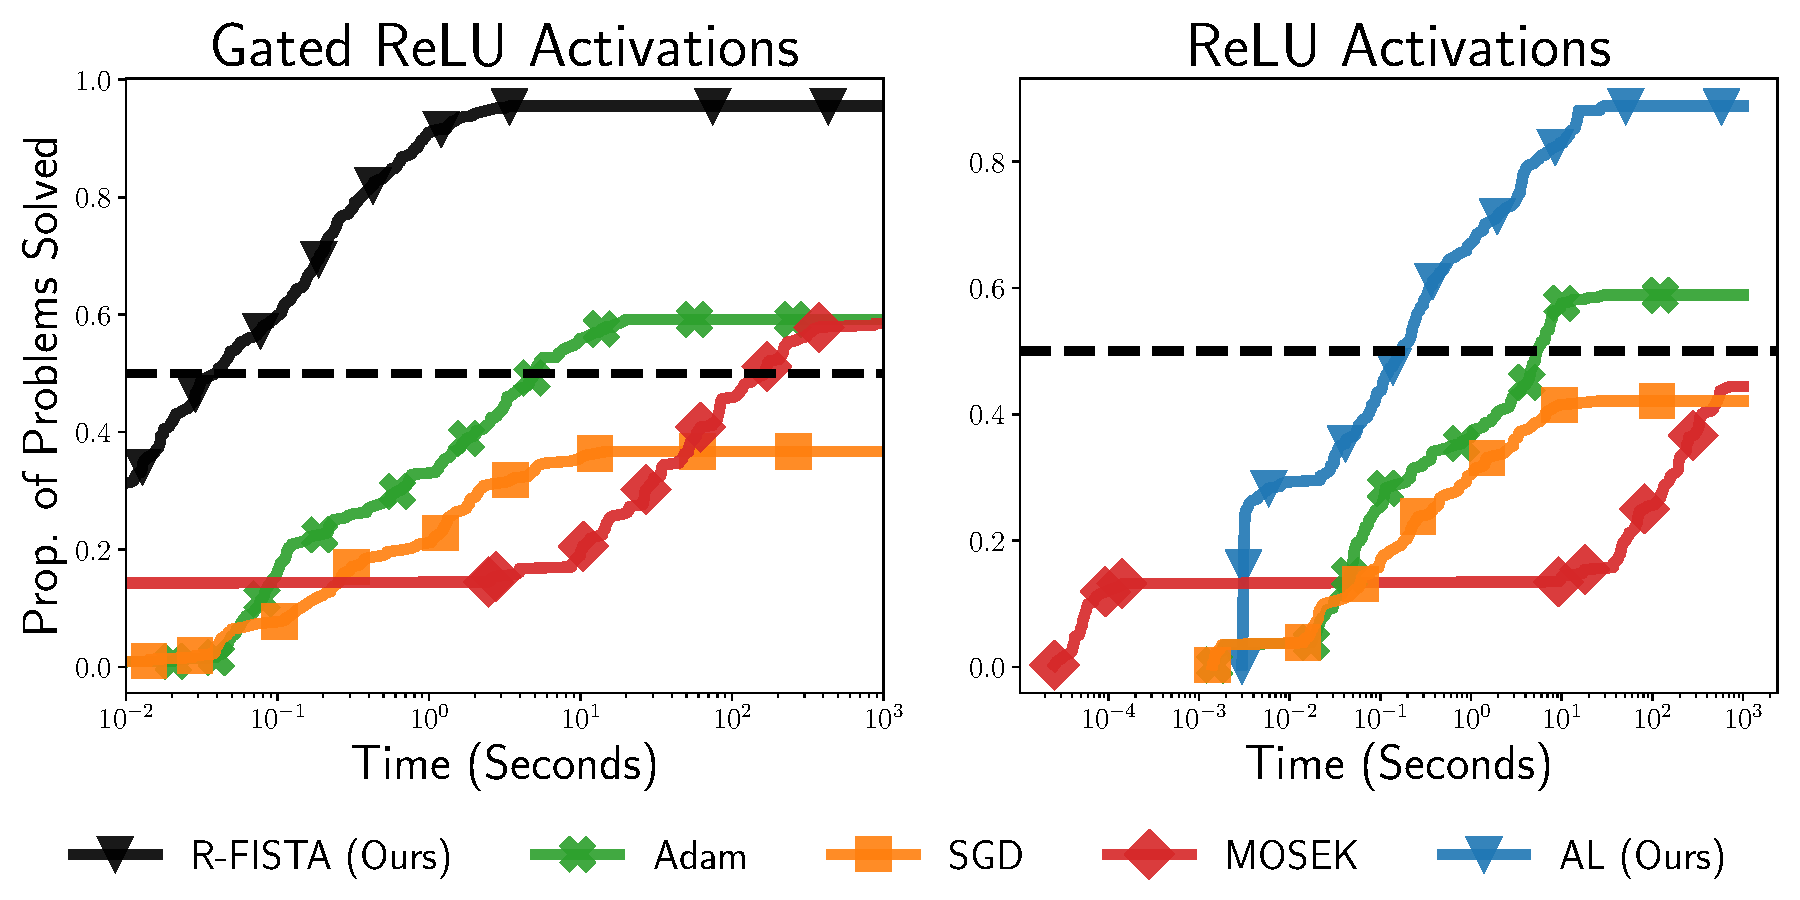
\includegraphics[width=0.96\linewidth]{figures/chapter_two/additional_pp/pp_main_05.pdf}
	\caption{
		Alternative version of \cref{fig:performance-profiles} with success threshold set to be \( r_{\text{gap}} = 0.5 \).
		Recall that a problem is considered solved when \( \rbr{F(x_k) - F(x^*)}/F(x^*) \leq r_{\text{gap}} \), where \( F(x^*) \) is the smallest objective value found by any method.
		We find that tightening the success threshold (as compared to \cref{fig:performance-profiles}) only improves the performance of our convex solvers relative to Adam and SGD.
	}%
	\label{fig:pp-main-05}
\end{figure}

\begin{figure}
	\centering
	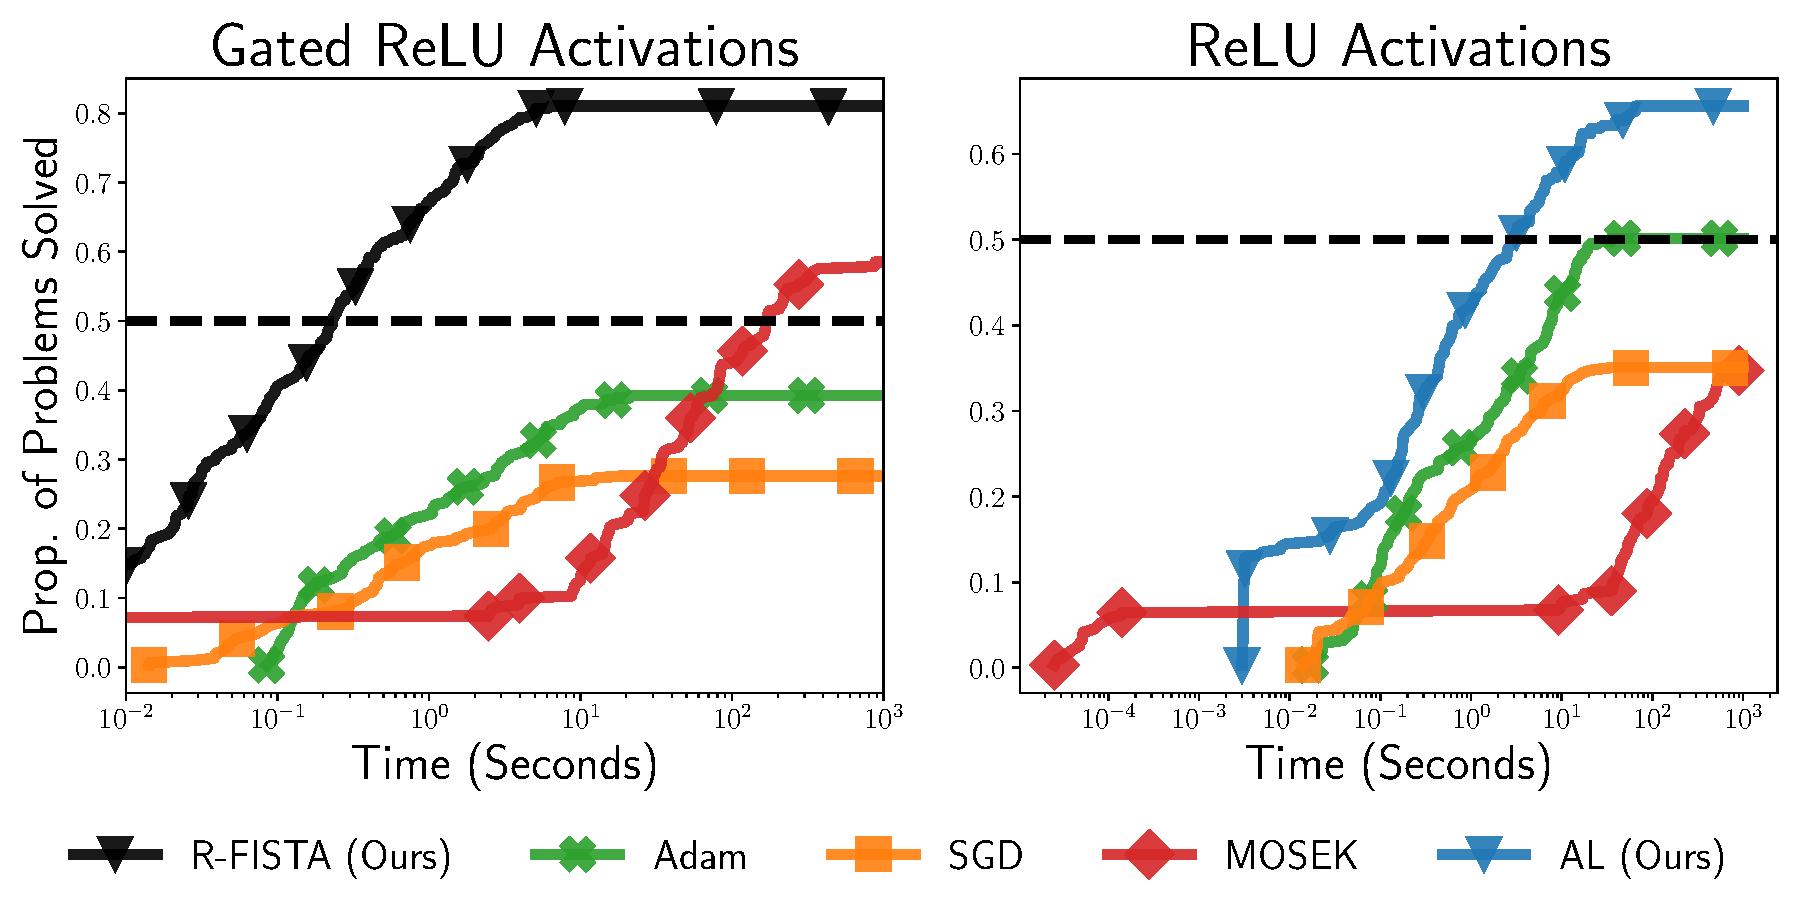
\includegraphics[width=0.96\linewidth]{figures/chapter_two/additional_pp/pp_main_01.pdf}
	\caption{
		Alternative version of \cref{fig:performance-profiles} with success threshold set to be \( r_{\text{gap}} = 0.1 \).
		Performance of all optimization methods decreases at this threshold, with the notable exception of MOSEK for the C-GReLU problem.
		However, the relative ordering of R-FISTA, AL, Adam, and SGD remains unchanged.
		In other words, our optimizers applied to the convex reformulations still out-perform the non-convex baselines.
	}%
	\label{fig:pp-main-01}
\end{figure}

\textbf{Alternative Success Thresholds}:
Choosing the threshold for the relative optimality gap \( \Delta_k \) is subjective and can potentially favor some methods over others.
In this section, we show that alternative values of \( r_{\text{gap}} \) preserve the ordering of methods from \cref{fig:performance-profiles}.
In particular, tightening the threshold shows that our convex solvers are not only faster than the non-convex baselines, but also solve the optimization problems to greater accuracy.

Figures~\ref{fig:pp-main-05} and~\ref{fig:pp-main-01} present the same experimental results as in Figure~\ref{fig:performance-profiles} with \( r_{\text{gap}} = 0.5 \) and \( r_{\text{gap}} = 0.1 \), respectively.
They should be compared against the threshold value of \( r_{\text{gap}} = 1 \) used in the main paper.
These figures show that the relative performance of each optimization method remains unchanged as the threshold is decreased, with the notable exception of MOSEK.
This is because MOSEK uses a highly accurate, but slow, interior point method.
